% "Shell Programming" talk
% Copyright (C) 2008  Chris Lamb <chris@chris-lamb.co.uk
%
% Based on a template (C) 2007, 2008 Daniel Watkins <D.M.Watkins@warwick.ac.uk>
%                     (C) 2007, 2008 Chris Lamb <chris@chris-lamb.co.uk>
%
%  This program is free software; you can redistribute it and/or modify
%  it under the terms of the GNU General Public License as published by
%  the Free Software Foundation; either version 3 of the License, or
%  (at your option) any later version.
%
%  This program is distributed in the hope that it will be useful,
%  but WITHOUT ANY WARRANTY; without even the implied warranty of
%  MERCHANTABILITY or FITNESS FOR A PARTICULAR PURPOSE.  See the
%  GNU General Public License for more details.
%
%  You should have received a copy of the GNU General Public License
%  along with this program; if not, write to the Free Software
%  Foundation, Inc., 51 Franklin St, Fifth Floor, Boston, MA  02110-1301  USA

\documentclass{beamer}

\usepackage{beamerthemesplit}
\usetheme{Warsaw}

\usepackage{graphicx}
\usepackage{url} 

\usepackage{listings} 
\lstset{basicstyle=\ttfamily}


\title{Shell Programming}
\author[Chris Lamb, WUGLUG]{Chris Lamb\\Warwick University GNU/Linux User Group}
\date{20th February 2008
\newline
\newline
\tiny{The \LaTeX{} source code for this presentation is licensed under version 3 of the GNU General Public License.}}

\begin{document}

\frame{\titlepage}

%

\section{Shell scripts}
    \subsection{Shell programming != Bash programming}
        \frame {
            \frametitle{Shell programming != Bash programming}

            Firstly:

            \begin{itemize}
                \item Bash is an \emph{implemention} of a shell \pause
                \item There are lots of other shells out there \pause
                \item ..that are faster and better \pause
                \item It makes a difference, dammit.
            \end{itemize}
        }
    \subsection{Shell microbenchmarks}
        \frame {
            \frametitle{Shell microbenchmarks}

            \begin{tiny}
                \lstinputlisting{benchmark.txt}
            \end{tiny}

            \pause

            \begin{enumerate}
                \item Dash -- 3 seconds \pause
                \item Ksh -- 12 seconds \pause
                \item Zsh -- 14 seconds \pause
                \item Bash -- 24 seconds \pause
            \end{enumerate}

            (Poor benchmark; basically testing integer-string conversion)
        }

    \subsection{Why not write in X?}
        \frame {
            \frametitle{Why not just write scripts in X?}

            \pause

            \begin{description}
                \item[C] -- Simply re-implementing the UNIX tools \pause
                \item[Python] -- Python shell scripts are ugly \pause
                \item[Ruby] -- Ruby is ugly \pause
                \item[Haskell] -- Only for Reddit karma and Linspire \pause
                \item[Perl] -- Maybe
            \end{description}
        }

    %

\section{Writing robust scripts}

    \frame {
        \frametitle{Writing robust scripts}

        Robust scripts: \pause
    
        \begin{itemize}
            \item Handle errors gracefully \pause
            \item Are maintainable \pause
            \item Are portable \pause
            \begin{itemize}
                \item Don't use untested/volatile semantics \pause
                \item Helps maintainability
            \end{itemize}
        \end{itemize}
    }

    \subsection{\lstinline!set -e! and \lstinline!set -u!}
        \frame {
            \frametitle{\lstinline!set -e!}

            \begin{itemize}
                \item Exits script if any statement returns with non-zero status: \pause
                    \begin{small}
                        \lstinputlisting{sete-example.txt}
                    \end{small}
                \item Should be enabled on every script you write! \pause
                \item Exits with non-zero status itself - chain scripts together \pause
                \item Use \lstinline!stmt || true! when a command is allowed to fail
            \end{itemize}
        }
        \frame {
            \frametitle{\lstinline!set -e! (cont.)}

            \begin{itemize}
                \item Partially caught in pipes:
                    \begin{small}
                        \lstinputlisting{sete-example2.txt}
                    \end{small}
                    \pause
                \item Not inherited by subshells:
                    \begin{small}
                        \lstinputlisting{sete-example3.txt}
                    \end{small}
                \pause
                \item These are more examples of general shell behaviour than \lstinline!set -e!
            \end{itemize}
        }

        \frame {
            \frametitle{\lstinline!set -u!}

            \begin{itemize}
                \item Ensures statements return non-zero status when unset variable is used: \pause
                    \begin{small}
                        \lstinputlisting{setu-example.txt}
                    \end{small}
                \pause
                \item Catches typos and logic errors \pause
                \item Use with `\lstinline!set -e!' so script fails when used \pause
                \item Programatically detect unset variables with `\lstinline!\$\{VAR:-\}!' \pause
                \item Useful for simple argument parsing - just reference `\lstinline!\$1!' and script will fail if unset! \pause
            \end{itemize}
        }
    \subsection{Traps and locks}
        \frame {
            \frametitle{Traps}

            \begin{itemize}
                \item Specify a function to jump to when a signal is received \pause
                \item `\lstinline!DEBUG!' pseudo-signal received after every command \pause
                \item Extremely unportable semantics beyond simple usage! \pause
                \item Be especially careful doing things inside your trapped function
            \end{itemize}
        }
        \frame {
            \frametitle{Traps}

            Implementing `transactional' behaviour: \pause

            \begin{tiny}
                \lstinputlisting{traps.txt}
            \end{tiny}
        }
        \frame {
            \frametitle{Locks}

            Preventing (accidental) concurrent usage: \pause

            \begin{tiny}
                \lstinputlisting{locks.txt}
            \end{tiny}
        }
    \subsection{Bashisms}
        \frame {
            \frametitle{Bashisms}

            \begin{itemize}
                \item Using Bash specific syntax whilst using \lstinline!/bin/sh!
                    is an instance of a Bashism. \pause
                \item Common examples: \pause
                \begin{itemize}
                    \item `\lstinline![[ test ]]!' -- use `\lstinline![ test ]!' \pause
                    \item `\lstinline!==!' in a test -- use `\lstinline!=!' \pause
                    \item `\lstinline!function!' to define a function \pause
                    \item `\lstinline!source filename!' -- use `\lstinline!. filename!' \pause
                    \item `\lstinline!. command args!' (not supported)
                \end{itemize}
            \end{itemize}
        }
        \frame {
            \frametitle{Bashisms (cont.)}
                
            \begin{itemize}
                \item Less common examples: \pause
                \begin{itemize}
                    \item '\lstinline!read!' without a variable \pause
                    \item Esoteric variable expansions (replacements, etc.) \pause
                \end{itemize}
                \item Also applies to Zsh! (Table-tennis operator, etc.)
            \end{itemize}
        }
        \frame {
            \frametitle{Evil Bashisms}

            \center{ 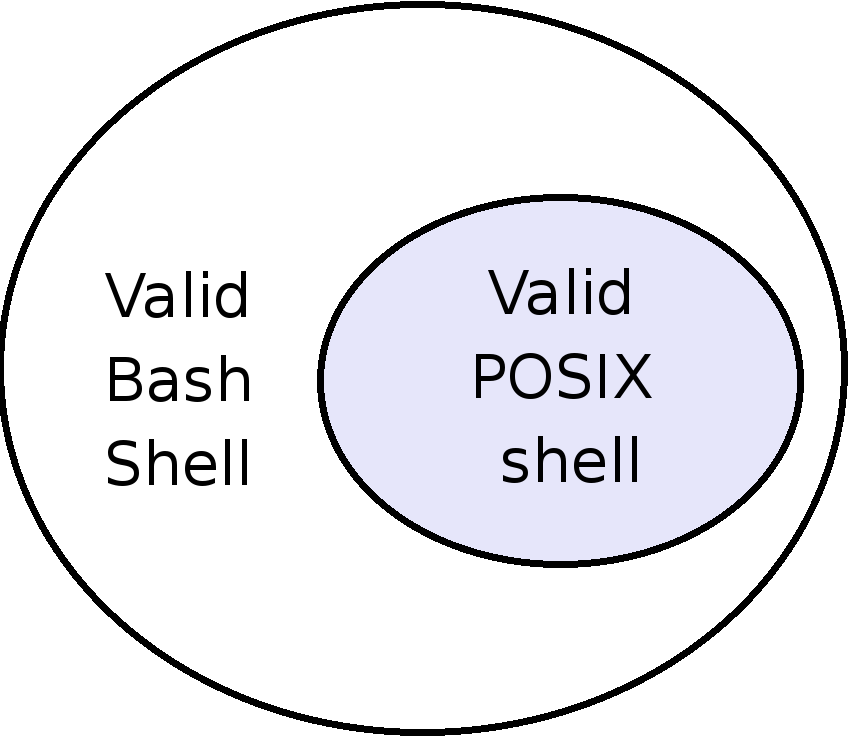
\includegraphics[width=60mm]{bashisms-superset.png} }

            Bash implements a superset of POSIX shell semantics and syntax...
        }
        \frame {
            \frametitle{Evil Bashisms (cont)}

            \center{ 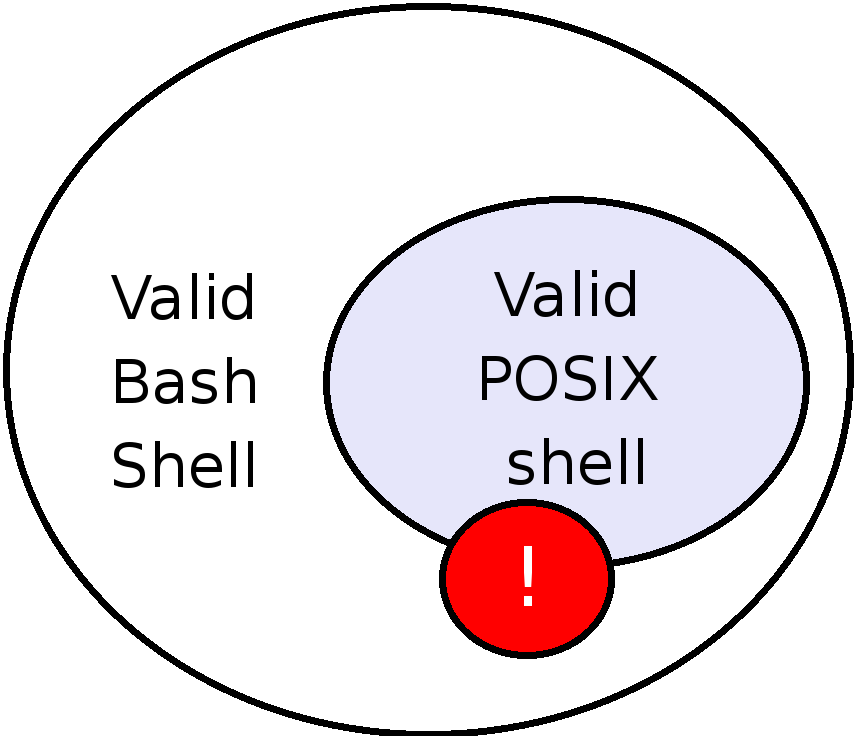
\includegraphics[width=60mm]{bashisms-evil.png} }

            .. but some Bash syntax has different semantics in POSIX shell!
        }
        \frame {
            \frametitle{Evil Bashisms (cont)}

            \begin{block}{`+=' unary operator}
                \lstinline!FOO+="BAR"!
                \begin{itemize}
                    \item In Bash -- appends the string ``bar'' to the variable \lstinline!FOO!
                    \item In POSIX shell -- runs the command ``\lstinline!FOO+="BAR"!'' !
                \end{itemize}
            \end{block} 

            \pause

            Plus others..
        }

    \subsection{Robust Makefiles}
        \frame {
            \frametitle{Robust Makefiles}

            \begin{itemize}
                \item Psuedo \lstinline!set -e!: \pause
                \begin{itemize}
                    \item Will fail on the third line:
                        \begin{tiny}
                            \lstinputlisting{makefiles-1.txt}
                        \end{tiny}
                        \pause
                    \item But what about:
                        \begin{tiny}
                            \lstinputlisting{makefiles-2.txt}
                        \end{tiny}
                    \pause
                    \item One solution is to add 'set -e' at the beginning of multi-line
                \end{itemize}
                \item No \lstinline!set -u! \pause
                \item \lstinline!\$(cmd)! already used, just ugly backticks \pause
                \item Scope of shell variables limited to single line
            \end{itemize}
        }
    \subsection{Misc.}
        \frame {
            \frametitle{Misc.}
            
            \begin{itemize}
                \item Set \lstinline!\$PATH! -- careful of trojans \pause
                \item Set \lstinline!\$IFS! -- security considerations \pause
                \item Spaces in filenames \pause
                \begin{itemize}
                    \item Can be dangerous! \pause
                    \item Experiment with \lstinline!strace -eexec -v! until you understand shell escaping \pause
                    \item Quoting variables is the usual solution \pause
                \end{itemize}
                \item \lstinline!\$\{FOO\}! vs \lstinline!\$FOO! \pause
             \end{itemize}
        }
%

\section{Shell toolbox}
    \frame {
            \frametitle{Shell toolbox}
            \pause
            \begin{itemize}
                \item UNIX has a ``software tools'' philosophy \pause
                \item Lots of smallish tools to perform a job
                \item `Shell' programming without tools is either useless or brain-damaged
            \end{itemize}
    }
    \subsection{\lstinline!sed! \& \lstinline!awk!}
        \frame {
            \frametitle{\lstinline!sed!}

            \begin{itemize}
                \item The Stream EDitor \pause
                \item \lstinline!echo hello | sed -e 's/hello/hi/'! \pause
                \item Powerful, but obscure syntax \pause
                \item Inline editing -- \lstinline!sed -i <expr> (<expr>)*! \pause
                \item `\lstinline!-n!' mode -- \lstinline!sed -n 's/search/replace/p'!
            \end{itemize}
        }
        \frame {
            \frametitle{\lstinline!awk!}

            \begin{itemize}
                \item Useful for record-oriented data \pause
                \item Lots of things are record-oriented \pause
                \item And even more things can be co-erced into being record-oriented! \pause
                \item \lstinline!cut -d: -f2! $\Leftrightarrow$ \lstinline!awk -F: '\{ print \$2 \}'! \pause
                \item \begin{small}
                    \lstinline!getent passwd | awk -F: '\$1 == "lamby" \{ print \$NF \}'!
                \end{small}
            \end{itemize}
        }
        \frame {
            \frametitle{Emulating other commands with \lstinline!awk!}

            \begin{description}
                \item[head] -- \lstinline!awk 'NR <= 10'! 
                \item[grep] -- \lstinline!awk '/regex/'!
                \item[wc -l] -- \lstinline!awk 'END \{ print NR \}'!
                \item[grep -v] -- \lstinline_awk '!/regex/'_
                \item[head -n1] -- \lstinline!awk 'NR > 1 \{ exit \}; 1'!
                \item[tail -n1] -- \lstinline!awk 'END \{ print \}'!
                \item[uniq] -- \lstinline!awk 'a \!\~ \$0; \{ a=\$0 \}'!
            \end{description}
        }
        \frame {
            \frametitle{An infamous example}

            \begin{tiny}
                \lstinputlisting{cp-progress-bar.txt}
            \end{tiny}
        }
    \subsection{\lstinline!echo! \& \lstinline!printf!}
        \frame {
            \frametitle{\lstinline!echo! \& \lstinline!printf!}

            \begin{itemize}
                \item \lstinline!echo! is really fragile and non-portable \pause
                \begin{itemize}
                    \item \lstinline!-e! or \lstinline!-n! not actually defined! \pause
                \end{itemize}
                \item Use \lstinline!printf! for reliable behaviour \pause
                \item \lstinline!printf! works well with \lstinline!xargs -L1! too
            \end{itemize}
        }
    \subsection{Processing arguments}
        \frame {
            \frametitle{Processing arguments}

            \begin{itemize}
                \item Easy to extend a script to accept multiple arguments \pause
                \item Existing script:
                    \begin{small}
                        \lstinputlisting{arguments-1.txt}
                    \end{small}
                    \pause
                \item Add \lstinline!while! and \lstinline!shift!:
                    \begin{small}
                        \lstinputlisting{arguments-2.txt}
                    \end{small}
            \end{itemize}
        }

    \subsection{Local variables}
        \frame {
            \frametitle{Local variables}

            \begin{itemize}
                \item Denote variables local to a function with `\lstinline!local!' \pause
                \item Values do not persist across invokations:
                    \begin{tiny}
                        \lstinputlisting{local-vars.txt}
                    \end{tiny}
                    \pause
                \item Locals usually in lowercase and globals in uppercase
                \pause
                \item Does not imply any sort of scoping!
            \end{itemize}
        }

    \subsection{\lstinline!find! and \lstinline!xargs!}
        \frame {
            \frametitle{\lstinline!find! and \lstinline!xargs!}

            \begin{itemize}
                \item Really useful \pause
                \item .. but dangerous! \pause
                \item Avoid \lstinline!find -exec! \pause
                \begin{itemize}
                    \item Don't forkbomb machines!
                \end{itemize}
                \item Be safe; use \lstinline!find -print0 | xargs -0!
            \end{itemize}
        }

\section{Debugging}
    \frame {
        \frametitle{Debugging}

        \begin{itemize}
            \item Check syntax with `\lstinline!/bin/sh -n!' \pause
            \item Debug specifics with `\lstinline!set -x!' (turn off with `\lstinline!set +x!') \pause
            \item \lstinline!checkbashisms! by Yann Dirson and Julian Gilbey
                (From \lstinline!devscripts! package on Debian - please port)
        \end{itemize}
    }

%

\frame {
    \frametitle{Thanks!}
    WUGLUG contact information:
    \begin{itemize}
        \item Website: \url{http://www.wuglug.org.uk}
        \item IRC: {\tt \#wuglug} on {\tt irc.uwcs.co.uk:6667}
        \item Mailing list: \url{https://mailman.warwickcompsoc.co.uk/listinfo/wuglug}
    \end{itemize}
}

\end{document}
